% =====================================================================
% Section V-B .. V-E, complete and corrected.
%
% Drop-in replacement for the four subsections: the brown draft with the
% hardware runs of HW_RUNS.md folded in, the shot count of the noise table
% fixed, and the two sentences that the runs require added to V-B and V-D.
% Delete the earlier copies of these subsections before including this.
%
% Every number is reproduced by the commands in HW_RUNS.md; SECV_HW_TEXT.md
% says which measurement backs which sentence.
% =====================================================================

\subsection{Zone-local distribution validation}
\label{subsec:eval_local_law}

The zone-local circuit is first validated independently of boundary coordination. Exact statevector simulation provides the complete outcome distribution without sampling or hardware noise, permitting a direct comparison with the analytical distribution in \eqref{eq:conditional-exponential}. Statevector memory grows exponentially with the qubit count, so this validation is limited to five zones of a small grid instance, with circuits reaching six UEs and 21 qubits. In every tested zone, the conditional distribution of the accepted outcomes agrees with \eqref{eq:conditional-exponential} to numerical precision, with a total-variation distance (TVD) below $3\times10^{-15}$, and no infeasible assignment appears among the accepted outcomes. The agreement verifies both parts of the construction: constraint evaluation excludes every assignment outside $\mathcal F_z$, and the utility rotations produce the intended relative probabilities among the feasible assignments. Across the same five zones, the marked probability $\mu_z$ in \eqref{eq:mu} decreases from $0.500$ to $0.017$ as the feasible set grows from one to $36$ assignments. Accepted samples therefore become harder to obtain as the zone grows, which is the reason for the execution budget and the local exponents introduced in Section~\ref{subsec:eval_setup}.

\begin{table}[!t]
\centering
\caption{Exact circuit checks of the assignment mechanisms. The first three circuits include one amplification round; the joint circuit checks preparation and constraint flags before amplification.}
\label{tab:eval_circuit_checks}
\footnotesize
\setlength{\tabcolsep}{3pt}
\begin{tabular}{lrrrr}
\toprule
Circuit & UEs & Qubits & $|\mathcal F|$ & TVD \\
\midrule
Inter-cell, unit demands & 4 & 16 & 6 & $2.2\times10^{-16}$ \\
Inter-cell, unequal demands & 4 & 16 & 10 & $2.8\times10^{-16}$ \\
Intra-cell, three RB candidates & 3 & 21 & 6 & $2.9\times10^{-16}$ \\
Joint, AP and RB limits active & 4 & 20 & 4 & $3.7\times10^{-15}$ \\
\bottomrule
\end{tabular}
\end{table}

Table~\ref{tab:eval_circuit_checks} adds three circuits that test mechanisms not exercised by the network instances, where every UE has a unit demand and at most two candidates. The inter-cell circuit is evaluated first with unit demands and AP capacity two, and then with demands $(1,2,1,2)$ and capacity four, so that the QFT adder accumulates demand rather than counting UEs. The intra-cell circuit gives each of three UEs three RB candidates with $W_r=1$; its two-bit index leaves one unused code, so agreement on the six feasible permutations also confirms that the invalid code is rejected. The joint circuit assigns four UEs to two APs that each own three RBs but admit only two UEs. Four of its $16$ candidate combinations satisfy the RB limits but violate an AP limit, and two satisfy the AP limits but violate an RB limit; the accepted distribution has support on exactly the four assignments that satisfy both. The same preparation, marking, and reflection structure therefore handles demand accumulation, invalid-code rejection, and simultaneous AP and RB limits. For the inter-cell and intra-cell circuits, the acceptance probability after one amplification round also agrees with \eqref{eq:success} within $10^{-12}$. In the unit-demand inter-cell circuit, acceptance rises from $0.0988$ to $0.6705$ while the conditional distribution remains unchanged, confirming that amplification increases the accepted mass without altering the utility weights within it.

\begin{table}[!t]
\centering
\caption{Inter-cell circuit under simulated noise, with $10{,}000$ shots per condition and one amplification round. TVD is computed after the decoded feasibility check.}
\label{tab:eval_noise}
\footnotesize
\begin{tabular}{lrr}
\toprule
Noise condition & Acceptance & TVD \\
\midrule
Noise-free & 0.666 & 0.005 \\
$p_2=10^{-4}$ & 0.650 & 0.011 \\
$p_2=10^{-3}$ & 0.513 & 0.016 \\
$p_2=10^{-2}$ & 0.104 & 0.137 \\
Calibration magnitudes & 0.123 & 0.134 \\
\bottomrule
\end{tabular}
\end{table}

Circuit behavior under hardware noise is evaluated with a simulated noise model. Table~\ref{tab:eval_noise} reports the four-UE inter-cell circuit under two noise settings. The controlled sweep applies a depolarizing error rate $p_2$ to two-qubit gates, $p_2/10$ to one-qubit gates, and a readout error of $p_2/5$. The last row instead uses the error magnitudes of the FakeSherbrooke calibration snapshot of a 127-qubit superconducting processor, whose median two-qubit, one-qubit, and readout error rates are $7.79\times10^{-3}$, $2.36\times10^{-4}$, and $1.98\times10^{-2}$. Both settings apply the noise to the qubits that the circuit uses, without routing onto the device coupling map, so they isolate gate and readout errors from routing overhead. Acceptance is the fraction of shots that pass the acceptance test of Section~\ref{sec:distribution}, and the TVD measures how far the accepted samples deviate from \eqref{eq:conditional-exponential}. The nonzero noise-free TVD comes from the finite number of shots.

At $p_2=10^{-3}$, acceptance decreases from $0.666$ to $0.513$ while the TVD stays close to its noise-free value. At the calibration magnitudes of the current device, acceptance drops to $0.123$ and the TVD rises to $0.134$, so the circuit needs about five times more executions per accepted sample and the utility weighting of the accepted samples is visibly distorted. Noise thus affects the sampling efficiency and the accuracy of the utility weighting, but not the feasibility of the reported samples. Feasibility is checked from the decoded assignment after measurement, independently of the internal flag states, and any measured assignment that violates the original constraints is discarded. This check is needed even without noise: one amplification round leaves some amplitude outside the accepted subspace, so $5.0\%$ of the noise-free outcomes pass the utility-qubit condition but decode to an infeasible assignment, and the proportion rises to $12.3\%$ at the calibration magnitudes. The decoded check therefore forms part of the acceptance test itself, and it keeps every reported sample feasible at the cost of some sampling efficiency.

Routing onto the device coupling map is evaluated separately by transpiling the complete $k=1$ circuits to the FakeSherbrooke basis and connectivity. The 16-qubit inter-cell circuit grows from $384$ to $969$ two-qubit gates and the 21-qubit intra-cell circuit from $1354$ to $3373$, about a factor of $2.5$ in both cases. The 2000-gate budget of Section~\ref{subsec:eval_setup} counts logical oracle gates before routing, so executing a budget-sized zone on a specific device requires this additional overhead to be taken into account. Both test circuits lie well below the budget, and the noise results above characterize the mechanism rather than a full-size zone circuit.

\begin{table}[!t]
\centering
\caption{Execution on ibm\_boston, $10{,}000$ shots per row, with exact values in parentheses. The $k=0$ rows carry no oracle and test the accepted law of \eqref{eq:conditional-exponential}; the $k=1$ rows add one amplification round. $P(\mathrm{opt})$ is the probability that an accepted sample is the optimal assignment.}
\label{tab:eval_hardware}
\footnotesize
\setlength{\tabcolsep}{3pt}
\begin{tabular}{lrrrr}
\toprule
Circuit & Routed 2q & Acceptance & TVD & $P(\mathrm{opt})$ \\
\midrule
$k=0$, three UEs & 6 & 0.298 (0.284) & 0.038 & 0.425 (0.436) \\
$k=0$, demands $(1,2,1,2)$ & 8 & 0.138 (0.141) & 0.049 & 0.436 (0.444) \\
$k=0$, six UEs & 8 & 0.139 (0.149) & 0.028 & 0.431 (0.423) \\
\midrule
$k=1$, three UEs & 364 & 0.337 (0.985) & 0.106 & 0.373 (0.436) \\
$k=1$, demands $(1,2,1,2)$ & 787 & 0.125 (0.838) & 0.159 & 0.299 (0.444) \\
$k=1$, same, no decoupling & 787 & 0.034 (0.838) & 0.437 & 0.079 (0.444) \\
$k=1$, six UEs & 1868 & 0.036 (0.860) & 0.248 & 0.222 (0.423) \\
\bottomrule
\end{tabular}
\end{table}

The same construction is executed on quantum processors: the superconducting devices ibm\_boston and ibm\_kingston, and the trapped-ion device IonQ Forte Enterprise, whose all-to-all connectivity needs no routing and executes the four-UE inter-cell circuit in $196$ two-qubit gates against $787$ after routing onto a heavy-hex lattice. Table~\ref{tab:eval_hardware} reports the runs on ibm\_boston, with $10{,}000$ shots each. Every reported assignment satisfies the original constraints, on every device and in every run, since the acceptance test is applied to the decoded assignment rather than to the internal flag states. Without amplification, the device reproduces the accepted law of \eqref{eq:conditional-exponential}: across six demand settings from three to six UEs, the TVD is $0.024$ to $0.049$, acceptance lands within $0.93$ to $1.07$ of its exact value, and the mean utility of an accepted sample is within $0.011$ of exact. The utility rotations of \eqref{eq:utility-angle} and the decoded acceptance test therefore operate as intended on hardware, and what the amplified rows add is the cost of the oracle itself.

Amplification is bounded by circuit size rather than by the construction. Over circuits of $364$ to $1868$ routed two-qubit gates, the marked branch decays by $0.0022$ to $0.0042$ per gate, which places the break-even of one round near $400$ routed gates, or about $355$ in the unrouted counting of \eqref{eq:zone_one_pass_cost}: a three-UE circuit of $364$ gates raises acceptance from $0.298$ without amplification to $0.337$ with it, whereas circuits of $580$ gates and above remain below their own baselines. Selection survives well past that point. At $1868$ routed gates, half the partition budget in the same counting, the surviving signal is $1.5\%$, yet the optimal assignment still holds $0.222$ of the accepted mass against $0.016$ for a random output, and five physical layouts of that circuit agree within $0.209$ to $0.251$.

What limits the executable size is circuit duration rather than gate count. The $787$-gate circuit loses its entire marked branch, from an acceptance of $0.125$ to $0.034$, when dynamical decoupling is disabled and its qubits idle through the same depth, while its gate count is unchanged. The simulated conditions of Table~\ref{tab:eval_noise} model gate and readout errors, and measured against these runs a noise model carrying the device's own gate errors overestimates the surviving signal by a factor of $3.4$ at $364$ routed gates and $55$ at $1868$, because the loss that grows with circuit size is this idling. The partition budget consequently bounds the circuit that a zone must fit into, which the zone circuits of Section~\ref{subsec:eval_network} meet in qubit width at $37.7$ to $43.0$ qubits against the $156$ of the devices used here, rather than the size at which a present device returns an undistorted accepted law.

Direct quantum simulation becomes impractical for the larger instances used in the region-scale experiments. An equivalent classical sampler is used to reproduce the zone-local distribution at these scales. Before feasibility screening, the state preparation $\mathcal P_z$ in \eqref{eq:op-prep} factorizes over the UE assignments, permitting independent utility-weighted candidate sampling. Applying the same feasibility conditions gives the accepted distribution $p_z$ in \eqref{eq:conditional-exponential}, and the exact agreement reported above justifies this substitution. The classical sampler replaces the physical generation of the local samples while preserving the distribution supplied to the coordination procedure. Circuit execution costs are still evaluated from $K_z/P_z(k)$ and do not correspond to measured classical runtimes.

\subsection{Boundary coordination in a partitioned region}
\label{subsec:eval_snapshot}

Fig. \ref{fig:snapshot} illustrates the complete distributed procedure for one campus instance with $M=25$ APs and $N=50$ UEs. The $2000$-gate partition produces $|\mathcal Z|=14$ zones and $|\mathcal B|=23$ boundary UEs, and the largest zone oracle uses $1910$ two-qubit gates. Boundary coordination involves $46\%$ of the UEs in this instance, so nearly half of the assignments are decided across zones rather than within one. The instance thus exercises the coordination procedure rather than reducing to independent local problems.

The representative local samples closely follow their exact accepted distributions despite the finite sample size. Assignments with larger $J_z$ occur more frequently according to the exponential utility weighting, while infeasible assignments receive no accepted probability. At $K_z=200$, the largest TVD between the sampled and exact distributions is $0.184$, with a mean of $0.115$ over the fourteen zones. In this instance, the local sampling exponents $\beta_z$ range from $1.36$ to the common target of $1.50$, and at least $198$ of the $200$ samples remain effective in every zone after reweighting, so the boundary decisions below rest on essentially the full sample sets. Larger reductions occur in the region-scale experiments of Section~\ref{subsec:eval_network}, where $\beta_z$ reaches $0.38$ and the effective sample size falls to $88$; their effect on solution quality is examined at the end of this subsection.

The same instance demonstrates why the joint structure of the local samples is preserved during coordination. For the two boundary-UE pairs with the strongest dependence, independently combining their UE-wise marginals assigns $19\%$ of the resulting probability mass to joint candidate choices that violate a local capacity constraint and do not occur in the feasible sample set. Each UE of such a pair can use a shared RB with positive probability, but the two cannot use it simultaneously under $W_r=1$. Positive individual marginals therefore do not imply that the corresponding joint choice is locally feasible, because neighboring UE assignments are coupled through the resource constraints. Fixed marginal distributions lose this dependence, whereas the feasible joint samples retain it.

Confidence-ordered decimation preserves this dependence by filtering the joint samples after each boundary decision and recomputing the remaining marginal and consensus distributions. A one-pass baseline instead computes the consensus distributions once and fixes all boundary UEs without re-conditioning the joint samples. Both variants use the same feasibility safeguards and selective re-sampling of Appendix~\ref{app:decimation}, so the comparison isolates the effect of re-conditioning. Across $14$ campus instances of intermediate size, re-conditioning gives a higher final utility in $11$ cases and improves the achieved fraction of $J^\star$ by $0.87$ percentage points on average, with a median of $0.53$ and a range from $-2.36$ to $+3.42$. The gain is not guaranteed on every instance, but on average the retained dependence leads to a better final assignment. The confidence values in Fig. \ref{fig:snapshot} decrease as less decisive boundary UEs are processed, and five selective re-sampling events replenish affected zones when their effective sample sizes become insufficient.

The final coordinated assignment for the campus instance satisfies all local capacity and boundary consistency conditions and achieves $98.66\%$ of the centralized optimum $J^\star$, computed exactly by the HiGHS integer-programming solver \cite{highs}. The instance belongs to a family of $16$ seeds on the same map, $13$ of which admit a globally feasible assignment. Across those $13$ instances, the achieved utility ranges from $97.34\%$ to $99.97\%$, with a mean of $99.19\%$. No instance reaches $J^\star$ exactly, so the residual gap of about one percentage point is a property of the procedure rather than of one particular draw. Joint-sample re-conditioning maintains the dependencies imposed by the local constraints while producing globally feasible assignments with utility close to the centralized optimum.

\begin{table}[!t]
\centering
\caption{Effect of the execution budget on 16 grid instances at the common target $\beta=1.5$. The report cost includes re-sampling requests.}
\label{tab:eval_budget}
\footnotesize
\setlength{\tabcolsep}{3pt}
\begin{tabular}{lrrr}
\toprule
Budget & Largest report & Mean utility & Worst loss$^a$ \\
 & executions & $J/J^\star$ [\%] & [pp] \\
\midrule
Unrestricted & $2.84\times10^7$ & 99.16 & 0.00 \\
$10^4$ & $10^4$ & 99.21 & 0.74 \\
$10^3$ & $10^3$ & 99.32 & 0.74 \\
\bottomrule
\end{tabular}
\par\smallskip
\parbox{\columnwidth}{\footnotesize $^a$Largest utility loss on any single instance relative to sampling at the target exponent without a budget. Execution counts are expected values.}
\end{table}

Table~\ref{tab:eval_budget} examines the execution budget of Section~\ref{subsec:eval_setup} on $16$ grid instances with $281$ zones in total. Because $\mu_z$ varies by orders of magnitude across zones, requesting $200$ samples at the target exponent without a budget would require up to $2.84\times10^7$ expected executions from a single zone. With the budget of $10^4$, the largest report costs $10^4$ executions, the mean utility is unchanged ($99.16\%$ against $99.21\%$), and the largest loss on any single instance relative to unbudgeted sampling is $0.74$ percentage points; the smallest effective sample size is about $87$ of $200$. A budget of $10^3$ gives similar results, and all $16$ instances remain feasible under every budget. Reducing the local exponent and reweighting therefore lowers the sampling cost by three orders of magnitude with only a small worst-case effect on the coordinated assignment. The mean utility does not improve with a smaller budget in any systematic way; the small differences reflect sample-to-sample variation of the sequential decisions.

\subsection{Zone-local circuit cost and latency}
\label{subsec:eval_local_scaling}

\begin{figure}[!t]
    \centering
    \includegraphics[width=\columnwidth]{fig/fig8}
    \caption{Modeled zone-local runtime against zone size for the
    proposed oracle and reference methods.}
    \label{fig:zone_crossover}
\end{figure}

Two-qubit gates dominate error accumulation and execution cost in quantum circuits. The two-qubit gate count and circuit depth of one oracle pass are used as the corresponding cost and latency measures. For zone $z$, let $D_z=\sum_{i\in\mathcal U_z}|\mathcal C_i|$ denote the number of evaluated candidate edges, $\ell_{\max,z}= \max_{i\in\mathcal U_z}\lceil\log_2|\mathcal C_i|\rceil$ the widest candidate index, $Q_z^{\mathrm{cnt}}$ the counter width in \eqref{eq:counter-width}, and $\mathcal M_z$ the set of capacity constraints evaluated in that zone. With approximate-QFT arithmetic \cite{coppersmith1994} and standard multi-control decompositions \cite{maslov2016}, both modeled depth $T_z$ and two-qubit gate count $G_z$ of oracle $\mathcal O_z$ scale as
\begin{equation}
T_z,\;G_z=O\!\left(D_z\left(\ell_{\max,z}+Q_z^{\mathrm{cnt}}\right)+|\mathcal M_z|Q_z^{\mathrm{cnt}}\right).
\label{eq:zone_one_pass_cost}
\end{equation}
Under bounded candidate degree and fixed counter width, both quantities grow linearly with the zone size. Parallel counters reduce the accumulation depth, while the remaining constraint and assignment operations set a floor on the achievable latency. Depth is also what limits the executable size on present hardware, as the decoupling comparison of Section~\ref{subsec:eval_local_law} shows, so reducing the accumulation depth is a present-device measure as well as a latency one.

Fig. \ref{fig:zone_crossover} evaluates this scaling with $D_z=2N_z$, $Q_z^{\mathrm{cnt}}=3$, and $|\mathcal M_z|=N_z$. The serial implementation evaluates the capacity constraints using one counter. The enhanced implementation uses $R_{\mathrm{cnt}}=4$ counters in parallel and parallelizes the per-UE matching and utility operations. Circuit depth is converted to modeled latency using $t_{\mathrm{layer}}=12.5\,$ns per logical layer, following the surface-code cycle assumption in \cite{campbell2019}. The same timing model is applied to the proposed method, GAS, and QTG, and all three quantum curves are computed from their depth expressions rather than measured on transpiled circuits. Each method is charged one oracle pass, excluding repeated search rounds, accepted-sample repetitions, readout, queueing, and boundary coordination.

The classical reference is $\rho N_z^3\,$ns with $\rho=0.400$, within the $0.058$--$0.740$ range measured for the Hungarian method \cite{kuhn1955} in \cite{jang2025cqf}. This reference does not include the capacity constraints evaluated by the proposed oracle, making the comparison conservative in favor of the classical computation. The proposed oracle has a modeled latency of approximately $113N_z\,$ns per pass under the enhanced schedule and $381N_z\,$ns under the serial schedule. GAS and QTG incur approximately $331N_z$ and $500N_z\,$ns, respectively, together with a common $37.5N_z\log_2N_z\,$ns contribution from the register that accumulates the zone-wide objective. The proposed construction avoids this objective register by representing the real-valued utilities through utility-qubit rotations.

The enhanced proposed schedule crosses the classical reference at approximately $18$ UEs per zone, compared with $31$ for the serial schedule, $37$ for GAS, and $42$ for QTG. These crossover points depend on the classical coefficient: varying $\rho$ over the measured range moves the enhanced crossover between approximately $13$ and $45$ UEs. They characterize one modeled oracle pass under the same fault-tolerant timing assumption. Repeated search rounds, accepted-sample repetitions, readout, queueing, and boundary coordination are outside this comparison. The crossover therefore characterizes oracle-level scaling rather than an end-to-end quantum speedup.

\subsection{Region-scale scalability}
\label{subsec:eval_network}

\begin{figure}[!t]
    \centering
    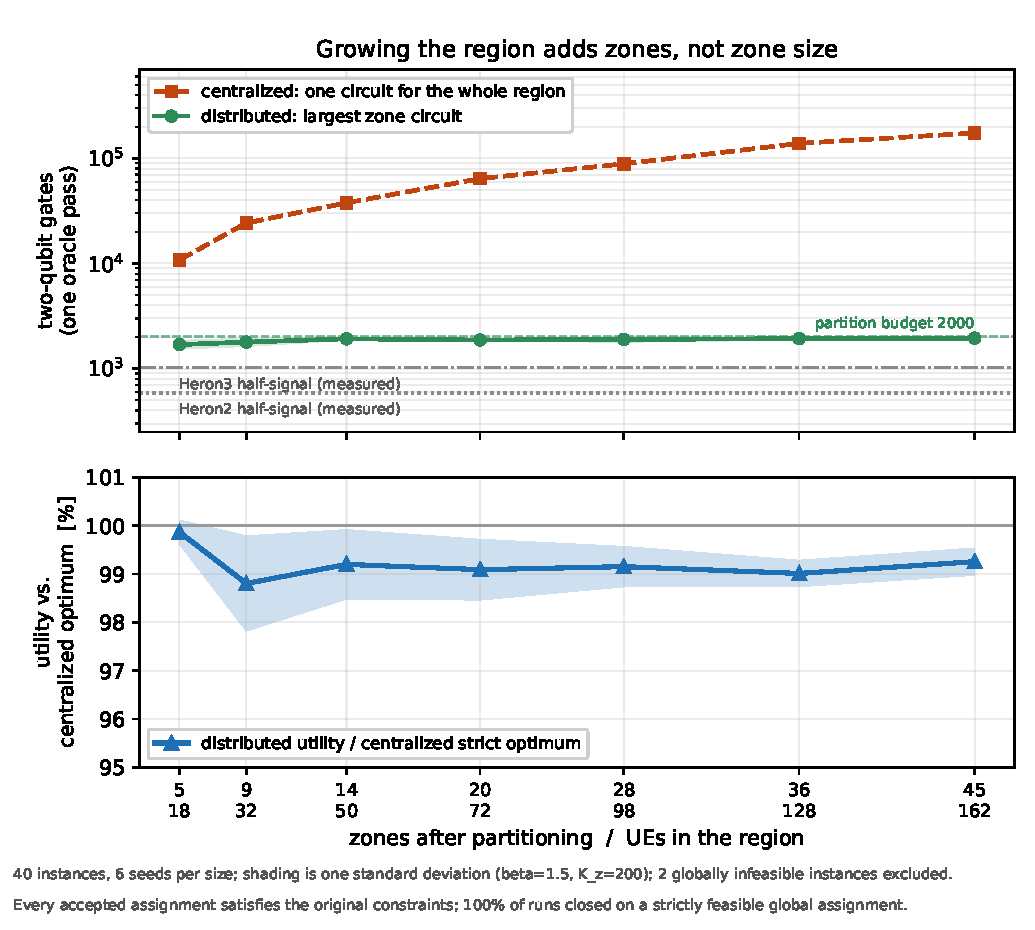
\includegraphics[width=\columnwidth]{fig/fig_scaling}
    \caption{Scaling of circuit complexity, coordination traffic, and
    solution utility with network region size.}
    \label{fig:region_scaling}
\end{figure}

The region-scale experiment examines how local quantum-resource demand, coordination traffic, and assignment quality change as the network expands. The sampled region is varied over seven sizes with six instances at each size. Two of the $42$ instances admit no globally feasible assignment and are excluded, leaving $40$ instances. The networks span $N=18$ to $N=162$ UEs, while the partition produces an average of $5.3$ to $45.0$ zones at fixed deployment density. Fig. \ref{fig:region_scaling} summarizes the resulting circuit complexity, communication volume, and utility.

A single circuit representing the entire region grows from $10{,}801$ to $173{,}983$ two-qubit gates over the evaluated range, an increase by a factor of $16$. In contrast, the largest zone circuit grows from $1{,}693$ to $1{,}950$ gates, a factor of only $1.15$, and never exceeds the 2000-gate partition budget for any region size. The qubit count shows the same behavior: the widest zone circuit grows from $37.7$ to $43.0$ qubits, a factor of $1.14$, whereas a single circuit for the entire region grows from $100.8$ to $828.3$ qubits, a factor of $8.2$. Increasing the covered region introduces additional bounded-size zones rather than proportionally enlarging the circuit executed within each zone. Under fixed deployment density, the quantum-resource demand of an individual zone, in both gate count and qubit count, remains nearly unchanged as the overall network expands.

For a zone with $n_z^{\mathrm{re}}$ re-sampling events, the coordination traffic is $(1+n_z^{\mathrm{re}})K_z (\sum_{i\in\mathcal B_z} \lceil\log_2|\mathcal C_i|\rceil+32)$ bits. The 32-bit field carries $J_z$ for the sample reweighting in \eqref{eq:app-reweight}. As the average number of zones increases by a factor of $8.4$, the total regional traffic increases by a similar factor of $9.0$. The mean communication volume per zone increases by only $6\%$. Re-sampling follows the same pattern: the mean number of re-sampling events per zone stays between $0.46$ and $0.61$ across the seven region sizes, and every instance completes on its first coordination attempt. Network expansion increases aggregate traffic primarily through the number of participating zones, while the communication and re-sampling burden of an individual zone remains nearly constant.

The distributed scaling does not produce a corresponding degradation in assignment quality. The mean coordinated utility remains between $98.76\%$ and $99.32\%$ of the centralized optimum $J^\star$ across the seven region sizes, with no systematic decrease as the network expands. Individual instances range from $96.79\%$ to $100\%$, and all $40$ instances produce globally feasible assignments, so \eqref{eq:factorization} holds in every run. The approximately one-percentage-point difference from the centralized optimum reflects the combined effects of decomposition, finite sampling, and sequential boundary commitments and does not increase over the evaluated range.

The zone-local circuits reproduce the intended feasible utility-weighted distribution, in exact simulation and, without amplification, on a quantum processor, and hardware noise affects their sampling efficiency and utility weighting rather than the feasibility of the reported samples. Joint-sample coordination maintains the assignment dependencies across zone boundaries. Increasing the network region adds bounded-size local computations rather than enlarging the quantum circuit of each zone, with the per-zone communication load remaining nearly unchanged. The resulting assignments remain globally feasible and close to the centralized optimum across the evaluated network sizes. These results demonstrate network-scale assignment through distributed quantum computation and coordination under bounded local quantum resources, with the executable circuit size on present processors set by circuit duration and measured here at about $400$ routed two-qubit gates for one amplification round.
